\documentclass[oneside]{article}
\usepackage[latin1]{inputenc}
\usepackage[brazil]{babel}
\usepackage{graphicx}
\usepackage{listings}
\usepackage{xcolor}
\usepackage{amsmath}
\usepackage{hyperref}
\usepackage{url}
\usepackage{breakurl}
\usepackage[left=2.7cm, right=2.7cm, bottom=3cm]{geometry}
\usepackage{caption}
\usepackage{subcaption}
\usepackage{lipsum}
\usepackage{fancyhdr}
\usepackage{listing}
\usepackage{gensymb}
\usepackage{caption}

%\renewcommand*{\refname}{Refer�ncias Bibliogr�ficas}

\fancyfoot[c]{\thepage}
\fancyhead[ro,le]{}
\fancyhead[lo]{\leftmark}
\fancyhead[re]{\rightmark}

\lstset{%
	linewidth=\textwidth,%framed box is the text size 
	xleftmargin=.25in,
	xrightmargin=.25in, 
	frame=trbl, 
	columns=flexible, 
	captionpos=t, 
	upquote=false,
	basicstyle=\small\ttfamily,
	firstnumber=1,% 
	numberfirstline=false,% 
	numbers=left,%
	numberstyle=\tiny,% 
	stepnumber=5,%
	numbersep=5pt,% 
	backgroundcolor=\color{green!15},% 
	tabsize=4,% 
	keywordstyle=\color{green!65!black},% 
	commentstyle=\color{blue},% 
	stringstyle=\color{magenta},% 
	breaklines=true,% 
	emph={label},%
	abovecaptionskip=10pt,% 
	belowcaptionskip={\abovecaptionskip},%
	showstringspaces=false, 
	literate={�}{{\^{E}}}1
}%

\lstdefinestyle{code} {%
	basicstyle=\ttfamily\footnotesize,
	backgroundcolor=\color{blue!10},
	%escapeinside={@}{@},
	frame=single, 
	captionpos=t,
	upquote=false,
	numberfirstline=false,% 
	stepnumber=5,%
	tabsize=4,% 
	keywordstyle=\color{green!65!black},% 
	commentstyle=\color{blue},%
	stringstyle=\color{magenta},% 
	breaklines=true,% 
	emph={label},%
	abovecaptionskip=10pt,% 
	belowcaptionskip={\abovecaptionskip},%
}%

\title{\huge
	\vspace{40pt}
	Sistema de Banco de Dados de uma Escola
	\vspace{25pt}
}

\author{
	Gabriel Peixoto de Carvalho\\
	\texttt{gaburiero.c@gmail.com}\\
	\texttt{201106840010}
	\and
	Thiago Barros Coelho\\
	\texttt{tbarroscoelho@gmail.com}\\
	\texttt{201106840041}
}
\date{
\vspace{100pt}
\begin{table}[!h]
	\begin{tabular*}{.9\linewidth}{p{.45\linewidth}p{.45\linewidth}}
	& Projeto apresentado � disciplina Banco de Dados 
	como requisito de avalia��o.
	Professor: Eloi Favero.
	\end{tabular*}
\end{table}
\vfill
Bel�m -- Brasil\\
\vspace{2pt}
Julho/2015
}

\begin{document}
% capa ------------------------------------------------------------------------
\thispagestyle{empty}
\begin{center}
\includegraphics[width=.16\textwidth]{Figures/logo_ufpa}\\

\vspace{12pt}
\bf\large
UNIVERSIDADE FEDERAL DO PAR�\\\vspace{1.5pt}
INSTITUTO DE TECNOLOGIA\\\vspace{1pt}
FACULDADE DE ENGENHARIA DA COMPUTA��O E\\\vspace{1.5pt}
TELECOMUNICA��ES\\

\vspace{120pt}
{\Large
Somador Completo de N�meros de 8 bits com Sinal
}

\vfill
\normalsize
Bel�m -- Brasil\\
Junho/2015
\end{center}
%%% EOF %%%


% T�tulo e Pre�mbulo -----------------------------------------------------------
\newpage
\maketitle
\thispagestyle{empty}

% Sum�rio e Lista de Figuras ---------------------------------------------------
\newpage
\tableofcontents
\listoffigures

% Introdu��o enunciado da questao-------------------------------------------------------------------
\newpage
\pagestyle{fancy}
\begin{section}{Enunciado da Quest�o}
\textbf{Para o enunciado abaixo,}\\ 
\textbf{(a) fa�a um modelo conceitual baseado na abordagem Entidade e Relacionamentos
(E-R);  (feito a m�o entregar no dia)... }\\
\textbf{(b) desenhe no dB-designer com todos os campos e gere o esquema do BD (entregar
o esquema textual e diagrama E-R impresso). }\\ 
\textbf{(c) Crie um script para criar o BD no (Interbase ou MySQl...) e um script para
dar carga  com pelo menos 40 alunos/respons�veis 5 professores e duas turmas. E
fa�a todas as consultas em SQL (R1 at� R6), mostrando a sa�da.}\\

Considere uma escola de ensino fundamental. Nesta escola desejam-se informatizar
diversos procedimentos, sendo coletados os requisitos que seguem. Primeiro �
necess�rio um cadastro de pais (ou respons�veis). Cada aluno tem um respons�vel
(um dos pais, ou outra pessoa). Para o respons�vel � necess�rio ter ID, nome e
fone.  Todo respons�vel tem um endere�o (string20 e.g. "rua pio X, nro13").\\
Cada matr�cula de um aluno vale para o ano corrente. Para o aluno guarda-se o
nome e fone. Para cada aluno cria-se um ID (inteiro) que vale para todos os anos
que o aluno permanecer no col�gio. Al�m disso, anualmente, cada aluno recebe um
n�mero de matricula composto por (ano, s�rie, turma, n�mero seq��ncia). Exemplos
de n�meros de matricula 20083TA23, 20061TB05. Numa turma s�o aceitos no m�ximo
50 alunos.\\

S�o registrados os valores das provas bimestrais dos alunos (duas vezes por
semestre), por mat�ria (portugu�s, matem�tica, geografia, etc). Se o aluno tirar
nota inferior a 60 fica em recupera��o no final de cada semestre, recebendo a
nota da recupera��o, que substitui a menor nota dos dois bimestres. Devem ser
mantidos registros de todas as provas e recupera��es todas notas de uma mat�ria
s�o registradas nos campos (B1,B2,B3,B4,R1,R2: numeric(2)) para cada
matricula.\\

O sistema deve emitir folhas de freq��ncia (Rel 1), com nome do professor de
cada turma e dos alunos, e da identifica��o da sala (ex. S10, S15); emitir 3
relat�rios.  O sistema deve emitir os boletins de notas (Rel 2) bimestrais
(cumulativo para o ano) para cada aluno; emitir relat�rio de notas para 3
alunos; mostram-se as notas das provas, recupera��es e m�dias semestrais e
anuais. O sistema deve emitir um hist�rico cumulativo (Rel 3) para cada aluno
considerando os v�rios anos; emitir 3 hist�ricos.\\

Para os professores registram-se � necess�rio ter ID, nome e fone. S�o criados
relat�rios com os \textbf{totais (quantidade) de alunos de recupera��o de cada turma
(Rel 4)}, com objetivo de prover orienta��o pedag�gica para os alunos com pais.\\

O sistema tamb�m controla o pagamento da mensalidade de cada aluno. S�o emitidos
boletos \textbf{(Rel 5)}, com o endere�o do respons�vel; Emitir 2 boletos, com repons�vel
e endere�o e aluno. Para cada aluno devem ser registrados os valores mensais
pagos; \textbf{s�o registrados para cada ano os valores na base como (valorMens,
m1,m2,m3,m4,...m12:float);} meses s�o inicializados zerados, quando pagos
marca-se o valor pago; o vencimento � o dia 7 de cada m�s; � preciso registar a
data do pagto. No momento da matricula � definido o valor a ser pago (valorMens)
que pode ser reajustado durante o ano (somente o valor atual � registrado em
valorMens). A qualquer momento o respons�vel pode solicitar um "extrato" dos
valores pagos e/ou vencidos de um aluno, dentro de um ano (Rel 6); emitir o
comprovante de tr�s alunos. 

\end{section}
%https://en.wikipedia.org/wiki/Turing_machine
%https://pt.wikipedia.org/wiki/Hist�ria_da_computa��o
%%% EOF %%%


% Esquemas e scripts de cria��o e insercao no banco ------------------------------
\begin{section}{Metodologia}

\subsection{Modelo do Banco}
O modelo do banco foi mostrado em aula de laborat�rio pelo professor da
disciplina e segue abaixo.

\begin{figure}[!h]
    \centering
    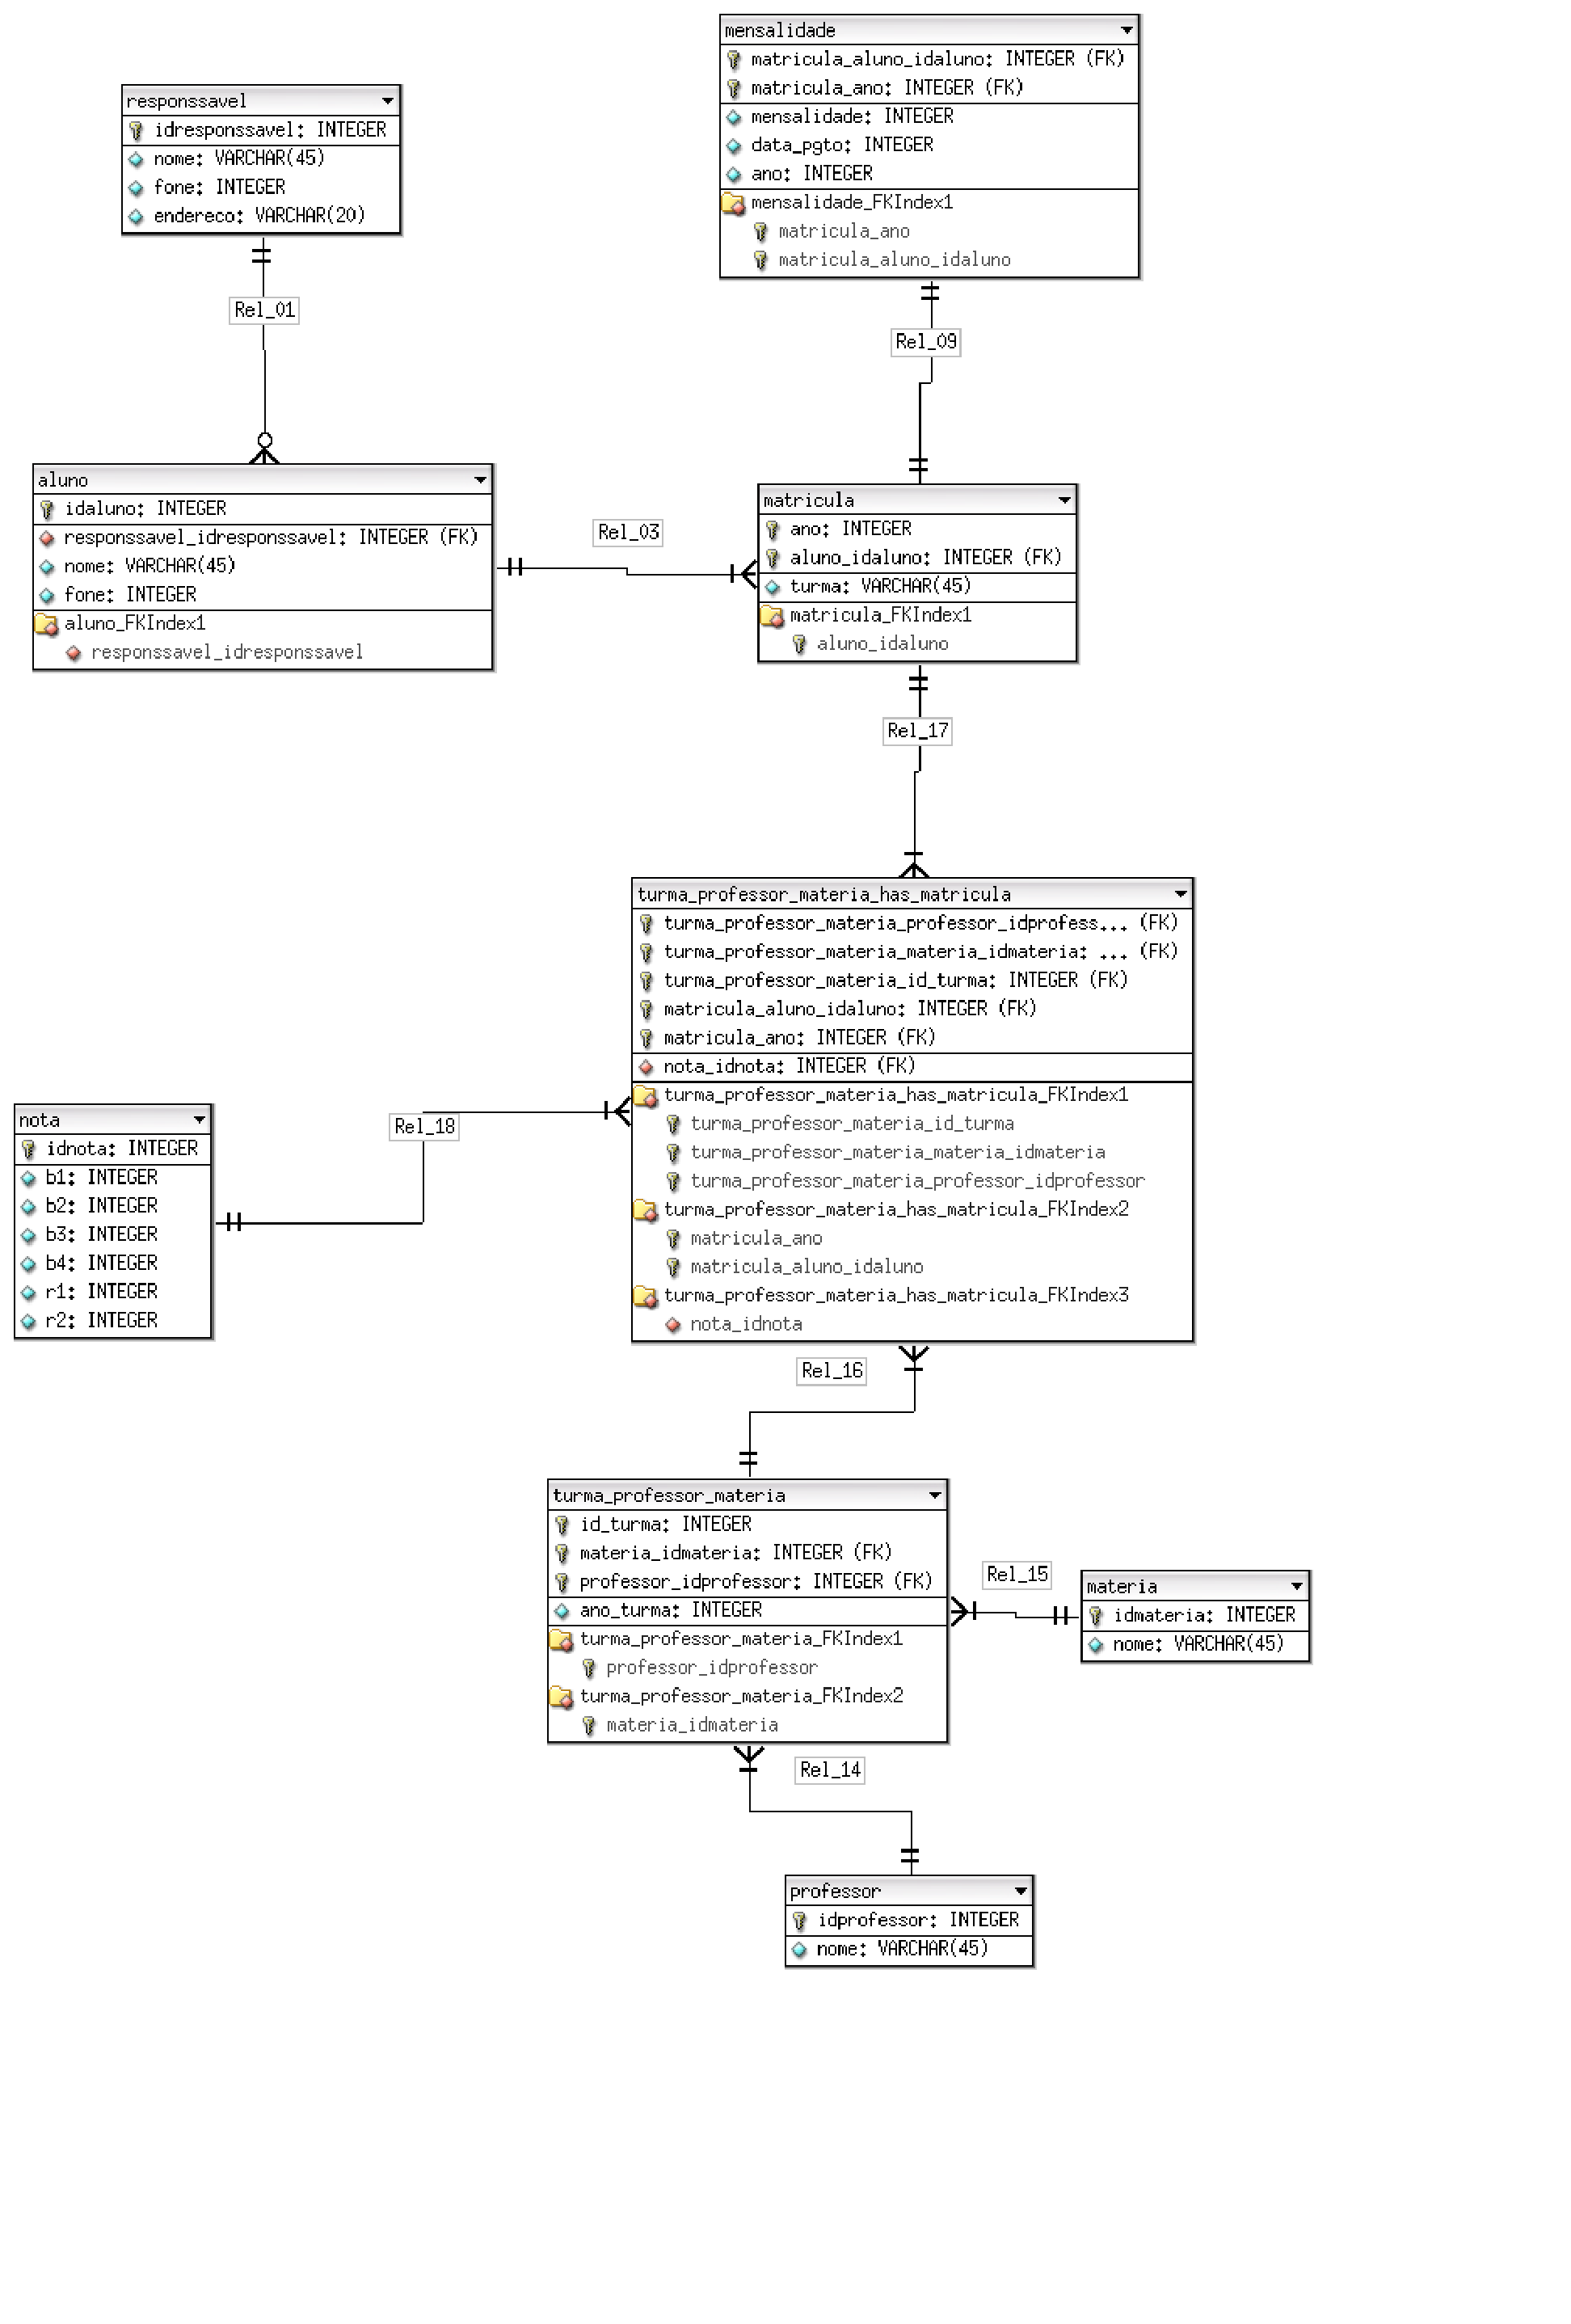
\includegraphics[width=.75\textwidth]{Figures/db_sch}
    \caption{Esquem�tio Entidade-Relacionamento}
    \label{fig:db_schema}
\end{figure}

\subsection{Cria��o do Banco}
A cria��o do Banco de dados foi feita como orientado pelo professor da
disciplina nas aulas de laborat�rio a partir do esquema \ref{fig:db_schema}feito no software
\textbf{DB Designer}.
\lstinputlisting[language=SQL]{../db_designer/db_escola_workbench_ver.sql}

\subsection{Inser��o de Valores}
A inser��o de dados no Banco foi feita como orientado no enunciado da quest�o.

\subsubsection{Respons�veis}
\lstinputlisting[language=SQL]{../db_designer/responsaveis_insertion.sql}

\subsubsection{Alunos}
\lstinputlisting[language=SQL]{../db_designer/alunos_insertion.sql}

\subsubsection{Professores}
\lstinputlisting[language=SQL]{../db_designer/professor_insertion.sql}

\subsubsection{Mat�rias}
\lstinputlisting[language=SQL]{../db_designer/materia_insert.sql}

\subsubsection{Forma��o das Turmas}
\lstinputlisting[language=SQL]{../db_designer/turma_professor_materia_insert.sql}

\subsubsection{Matr�cula}
\lstinputlisting[language=SQL]{../db_designer/Matricula_insert.sql}

subsubsection{Notas}
\lstinputlisting[language=SQL]{../db_designer/notas_insert.sql}

\subsubsection{Mensalidade}
\lstinputlisting[language=SQL]{../db_designer/mensalidade_insert.sql}

\end{section}

%%% EOF %%%


% Implementa��o: Funcionamento do circuito -------------------------------------
\begin{section}{Implementa��o}
O objetivo do trabalho � utilizar as ferramentas da fabricante Altera em
conjunto com o\textit{software} Quartus II. O kit de desenvolvimento
EP2C35F672C6 da fam�lia Cyclone II, mostrado na Figura~\ref{fig:cyclone}, foi
utilizado como base do projeto. 

\begin{figure}[!h]
	\centering
	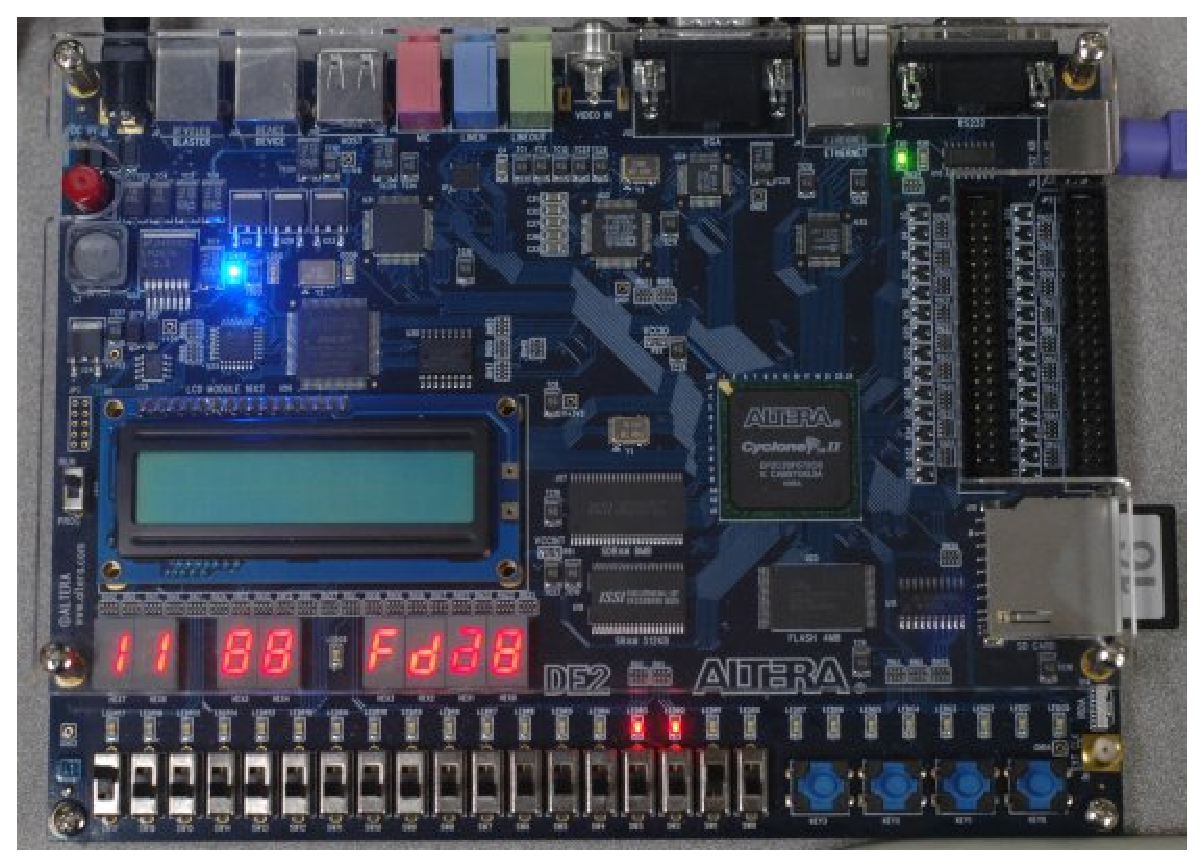
\includegraphics[width=.50\textwidth]{Figures/cyclone}
	\caption{DE Cyclone II EP2C35F672C6.}
	\label{fig:cyclone}
\end{figure}
A implementa��o do sistema foi feita em \emph{VHDL} no software 
\emph{QuartusII}, no qual foram impmentadas as rotinas de entrada/sa�da de dados
e todo o circuito l�gico respos�vel por converter a entrada para complemento de
2, somar e produzir uma sa�da decimal.
O desenvolvimento do sistema se deu da forma mais intuitiva o possivel,
componentes simples foram combinados em componentes mais complexos.

\subsection{Entrada de Dados}
A entrada de dados foi pensada de uma forma paralela, pois as chaves da placa de
desenvolvimento \emph{DE2} poderiam ser usadas como entrada. Para tornar o
processamento dessa entrada interna mais f�cil, os dados paralelos s�o
convertidos para uma sa�da vetorial.\\
%citar imagem com diagrama%
H� tamb�m outras entradas no sistema, como h� a necessidade de se somarem 3
n�meros, � preciso de duas chaves extras para sele��o de sa�da de um
demultiplexador modificado para o projeto onde a l�gica segue abaixo:

\begin{itemize}
    \item 00 - Primeiro n�mero;
    \item 01 - Segundo n�mero;
    \item 10 - Terceiro n�mero;
    \item 11 - Zera todas as entradas.
\end{itemize}

Al�m das chaves de sele��o h� uma chave para ser usada como \emph{clock enable} 
do \emph{Flip-Flop D}, o qual � a mem�ria do sitema.\\

C�digo de entrada de dados por chave:
\lstinputlisting[language=VHDL]{/home/gaburiero/git/phi-fulladder/src/parallel2serial8.vhd}

C�digo de entrada de chaves de sele��o:
\lstinputlisting[language=VHDL]{/home/gaburiero/git/phi-fulladder/src/parallel2serial2.vhd}

C�digo do demultiplexador modificado para o sistema:
\lstinputlisting[language=VHDL]{/home/gaburiero/git/phi-fulladder/src/demux3.vhd}


\subsection{Mem�ria}
A mem�ria do sistema � composta por 3 \emph{Flip-Flops D}, um para cada entrada.
Esses flip-flops necessitam de uma entrada de clock e uma de clock enable, como
explicado anteriormente, e ir�o guardar os dados at� que seja dado o comando de
soma. A implementa��o � como, citada anteriormente, parte de um flip-flop de um
bit e depois implementa um de 8 bits como mostrado nos codigos-fonte abaixo:

\lstinputlisting[language=VHDL]{/home/gaburiero/git/phi-fulladder/src/flipflop.vhd}

\lstinputlisting[language=VHDL]{/home/gaburiero/git/phi-fulladder/src/flop8.vhd}



\subsection{L�gica}
A l�gica do sistema consiste em:
\begin{itemize}
    \item Converter a entrada para bin�rio em complemento de 2;
    \item Fazer a soma em complemento de 2;
    \item Desconverter o complemento de 2 para nota��o bin�ria convencional;
    \item Converter a entrada bin�ria para \emph{BCD (binary coded
    decimal)}.
\end{itemize}

\subsubsection{Bloco Complemento de 2}
A convers�o em complemento de 2 como especificado em \ref{fig:complement2} �
realizada no c�digo exemplificado abaixo:

\lstinputlisting[language=VHDL]{/home/gaburiero/git/phi-fulladder/src/2complement.vhd}

Foi necess�rio o uso de um clock para sincronia de entrada e sa�da nesse
bloco.\\

\subsubsection{Bloco Somador de 8 bits}
A soma com complemento de 2 segue o mesmo algoritmo de uma soma com n�meros sem
sinal, mas na implementa��o do sistema deve-se salientar como o bloco somador
foi criado. Primeiramente, um bloco meio somador foi criado:

\lstinputlisting[language=VHDL]{/home/gaburiero/git/phi-fulladder/src/adder.vhd}

A partir de 2 meio somadores � poss�vel implementar um somador completo:\\

\lstinputlisting[language=VHDL]{/home/gaburiero/git/phi-fulladder/src/fulladder.vhd}

E finalmente, usando 8 somadores completos em paralelo � poss�vel implementar o
bloco somador de 8 bits do sistema. A linguagem VHDL permite usar uma clausula
\emph{generate} combinado com um \emph{loop} e mapeando a entrada vetorial para
cada porta de cada somador completo foi possivel criar um somador de 8 bits em
poucas linhas de c�digo, tal como mostrado abaixo:\\

\lstinputlisting[language=VHDL]{/home/gaburiero/git/phi-fulladder/src/8bitadder.vhd}

\subsubsection{Bloco Desconversor de Complemento de 2}
Ap�s o bloco somador � necess�rio converter o sinal gerado de volta para a
nota��o bin�ria usual e separar o bit de sinal para ser usado na sa�da no
display. Esse bloco � simplesmente o Inverso do \emph{bloco de complemento de
2}, como explicitado abaixo:\\

\lstinputlisting[language=VHDL]{/home/gaburiero/git/phi-fulladder/src/deconv.vhd}

\subsubsection{Bloco Conversor BCD}

A convers�o para BCD(\emph{Binary Doded Decimal}) � feita atrav�s do algoritmo
\emph{Double Dabble} como mostrado no c�digo-fone abaixo:\\

\lstinputlisting[language=VHDL]{/home/gaburiero/git/phi-fulladder/src/bin2bcd.vhd}

\subsection{Sa�da de Dados}
A sa�da de dados � realizada atrav�s dos displays de 7 segmentos na placa
\ref{fig:cyclone}, onde basicamente, o bloco decodificador recebe o bit de
sinal e a sa�da do conversor BCD, a partir da� os bin�rios s�o convertidos para
sa�das nos displays como mostrado abaixo:\\

\lstinputlisting[language=VHDL]{/home/gaburiero/git/phi-fulladder/src/disp7_8bit.vhd}


\end{section}
%%% EOF %%%


% An�lise e Simula��o: Modelsim ------------------------------------------------
\begin{section}{Resultados}

\subsection{Sa�da das Consultas}
\subsubsection{\textbf{Consulta 1}}
	Consulta da Folha de frequ�ncia de todos os estudantes (Figuras ~\ref{fig:r11}
e ~\ref{fig:r12}).
\begin{figure}[!h]
    \centering
    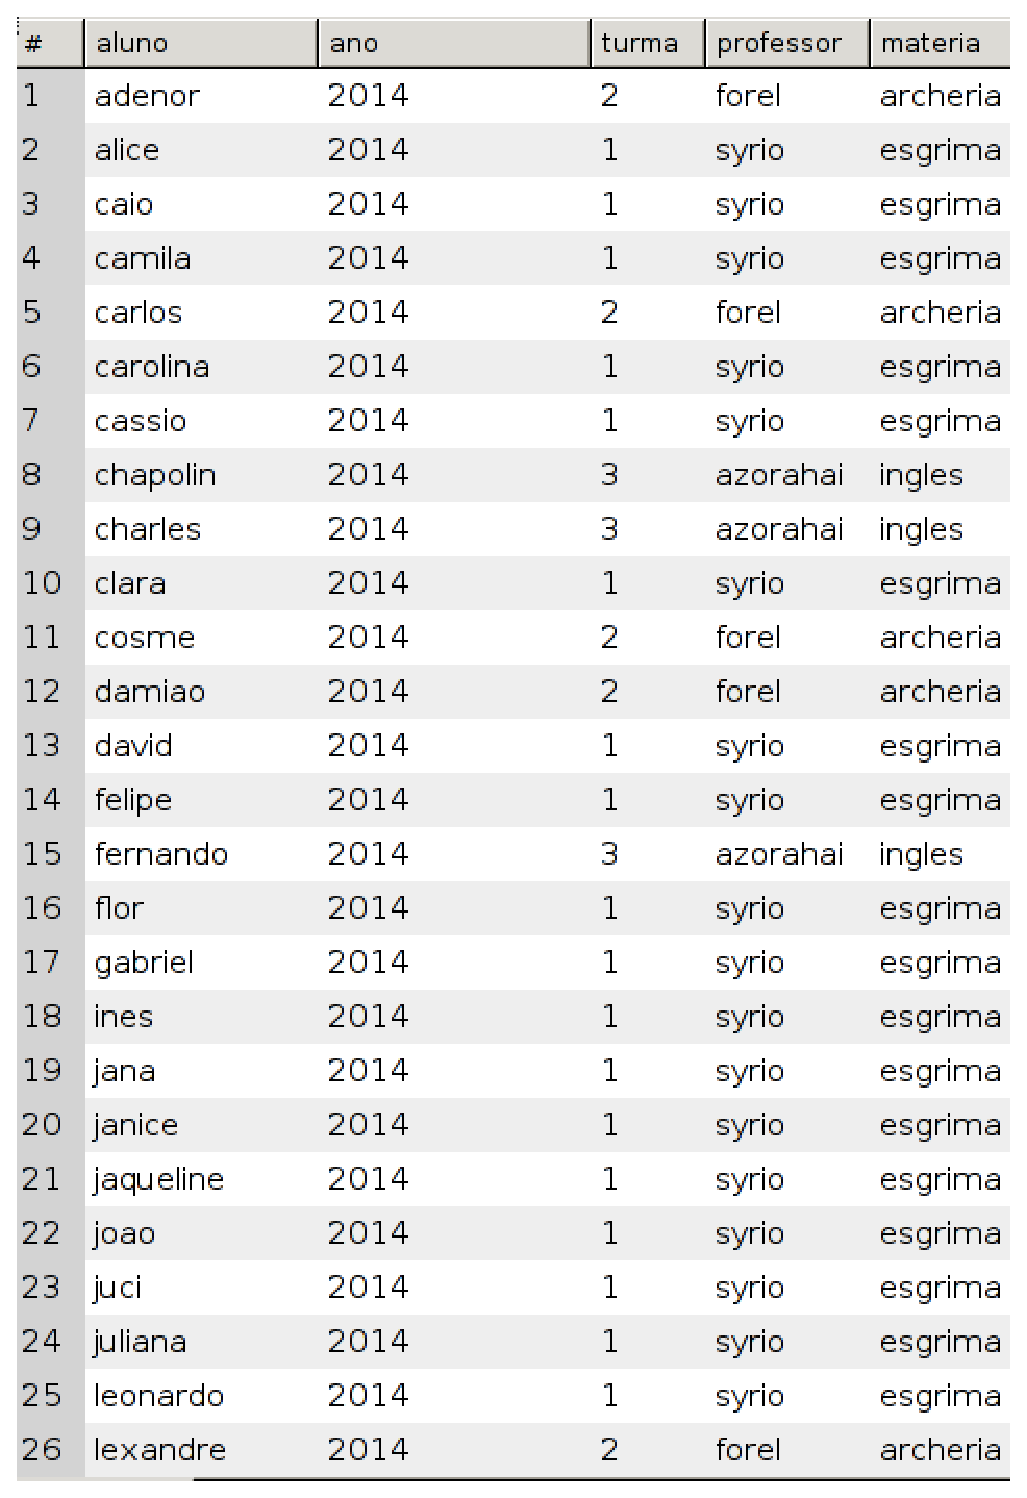
\includegraphics[width=.7\textwidth]{Figures/r11}
    \caption{Sa�da da Consulta 1 \textbf{parte 1}}
    \label{fig:r11}
\end{figure}

\begin{figure}[!h]
    \centering
    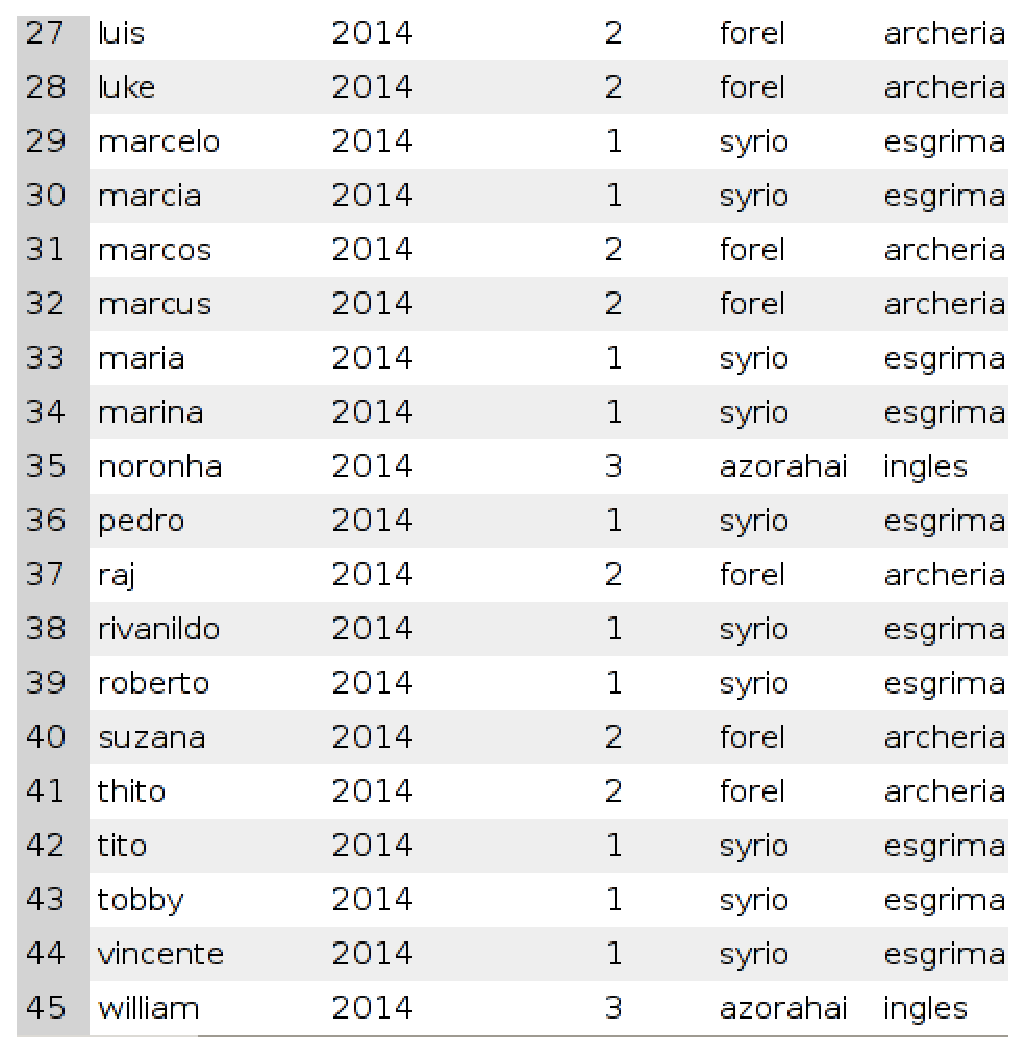
\includegraphics[width=.7\textwidth]{Figures/r12}
    \caption{Sa�da da Consulta 1 \textbf{parte 2}}
    \label{fig:r12}
\end{figure}

\subsubsection{\textbf{Consulta 2}}

	Boletim de notas de alguns estudantes (Figura ~\ref{fig:r2}).
\begin{figure}[!h]
    \centering
    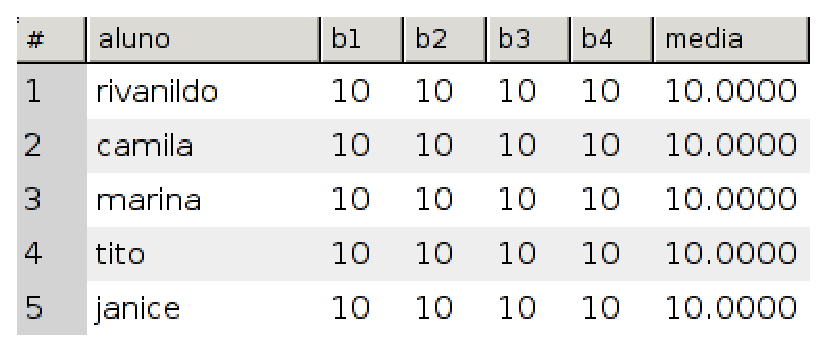
\includegraphics[width=.7\textwidth]{Figures/r2}
    \caption{Sa�da da Consulta 2}
    \label{fig:r2}
\end{figure}

\subsubsection{\textbf{Consulta 3}}
	Hist�rico cumulativo de alguns dos estudantes (Figura ~\ref{fig:r3}).
\begin{figure}[!h]
    \centering
    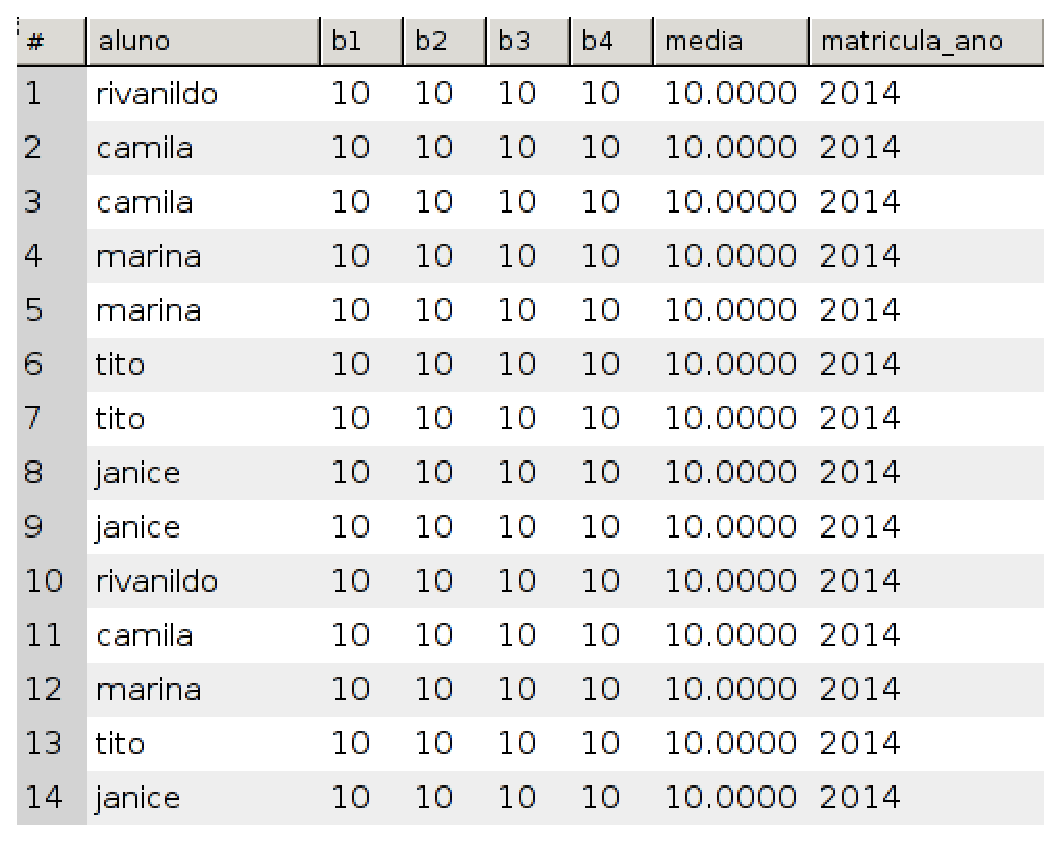
\includegraphics[width=.7\textwidth]{Figures/r3}
    \caption{Sa�da da Consulta 3}
    \label{fig:r3}
\end{figure}

\subsubsection{\textbf{Consulta 4}}
	Nome dos alunos em recupera��o por turma (Figura ~\ref{fig:r4}).
\begin{figure}[!h]
    \centering
    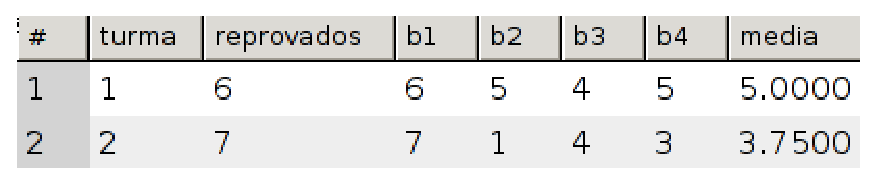
\includegraphics[width=.7\textwidth]{Figures/r4}
    \caption{Sa�da da Consulta 4}
    \label{fig:r4}
\end{figure}

\subsubsection{\textbf{Consulta 5}}
	Boleto mensal de (2) respons�veis (Figura ~\ref{fig:r5}).
\begin{figure}[!h]
    \centering
    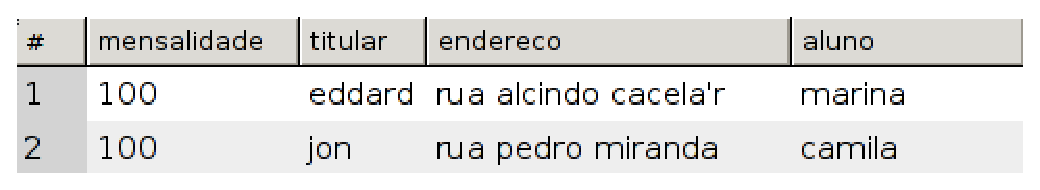
\includegraphics[width=.7\textwidth]{Figures/r5}
    \caption{Sa�da da Consulta 5}
    \label{fig:r5}
\end{figure}

\subsubsection{\textbf{Consulta 6}}
	Extrato anual de (3) alunos (Figura ~\ref{fig:r6}).
\begin{figure}[!h]
    \centering
    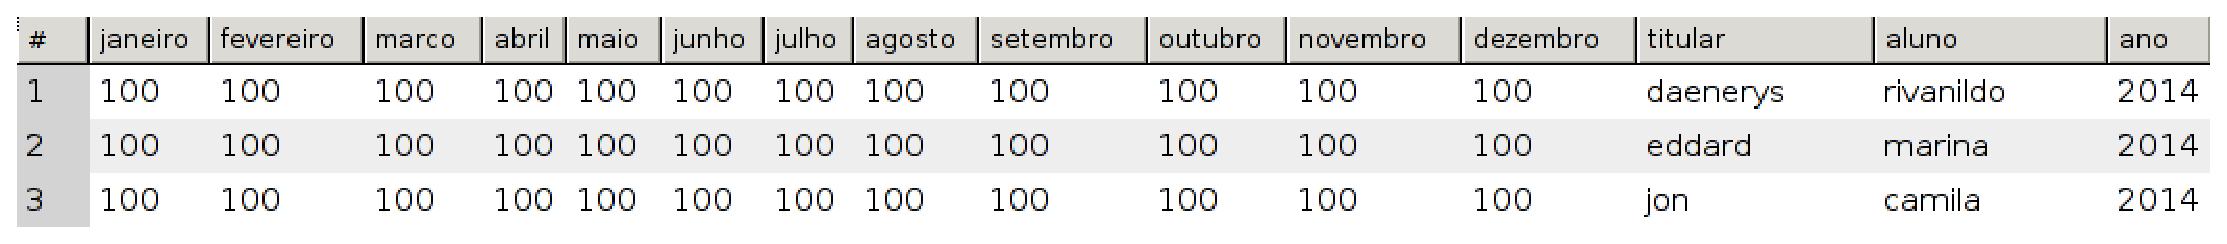
\includegraphics[width=.8\textwidth]{Figures/r6}
    \caption{Sa�da da Consulta 6 }
    \label{fig:r6}
\end{figure}


\end{section}
%%% EOF %%%


%\bibliographystyle{ieeetr}
%\bibliography{tech_report}

% C�digos e Background Matem�tico ----------------------------------------------
\newpage
\appendix
%\input{apendice}
\end{document}
%%% EOF %%%
